\documentclass[a4paper,10pt]{article}
\usepackage[utf8x]{inputenc}
\usepackage{graphicx}
\usepackage{pgf}
\pgfdeclareimage[height=1cm]{myimage}{p1_q1.png}


%opening   
\title{ \textbf{Universidade de Brasília -- Faculdade do Gama \\ Sistemas embarcados \\ Lista 2 }}
\date{Setembro - 2011}

\begin{document}
\maketitle

\section{Parte 1}
\begin{enumerate}
 \item Uma caldeira é uma máquina térmica utilizada na maioria das indústrias para a geração de vapor para outros equipamentos (como autoclaves, etc). 
      Sabe-se que para operar uma caldeira é necessário desenvolver um sistema de controle e monitoramento robusto, com tempo de resposta 
      determinístico por se tratar de um equipamento de alta periculosidade. Nesse sentido, é de fundamental importância que os parâmetros da 
      caldeira (temperatura, pressão interna e nível de água) sejam continuamente monitorados. Os sensores de temperatura, pressão e nível de água 
      estão conectados a um sistema de aquisição que converte os dados do mesmo e as transmitem para o painel de instrumentos da caldeira. As
      informações de pressão, temperatura e nível de água devem ser periodicamente atualizadas em um display em 500, 800 e 900ms respectivamente. 
      As informações são fornecidas pelo sistema de aquisição a uma taxa de 200ms e atualizadas conforme descrito acima. Com base nas informações 
      fornecidas:
\begin{figure}[ht]
 \center
 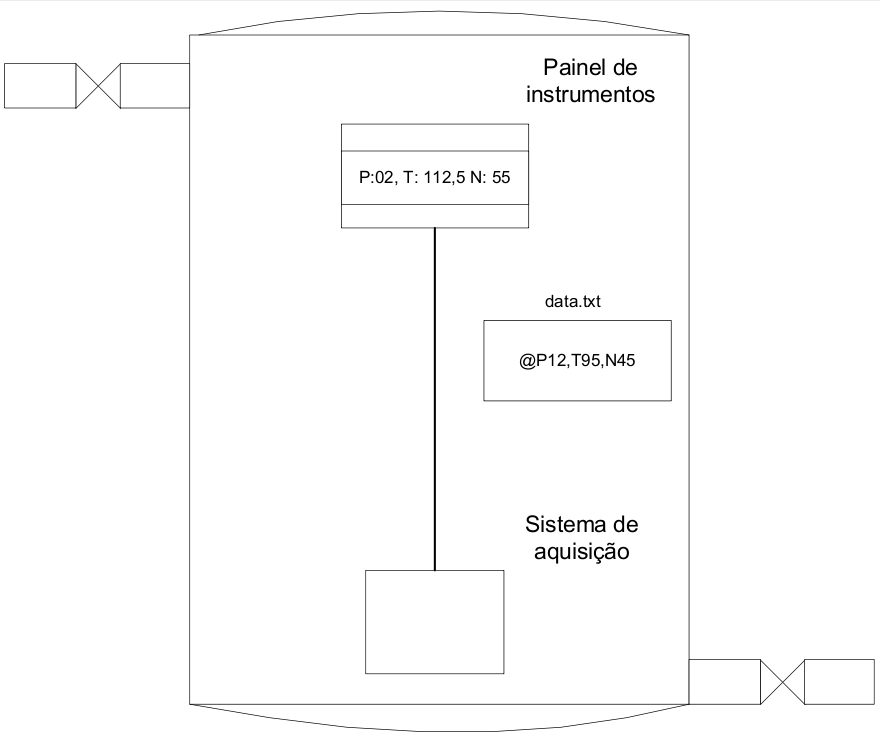
\includegraphics[width=10cm]{imagem/caldeira.png}
\end{figure}

\newpage

  \begin{itemize}
   \item Desenvolva um aplicativo que simule o funcionamento do sistema de aquisição de dados e do painel de instrumentos. Observe que os dados dos 
	sensores deverão ser lidos de um arquivo data.txt com o seguinte formato: @PXX,TXX,NXX em que XX representa as medições de pressão, 
	temperatura e nível de água respectivamente;
  \end{itemize}

  \item Um engenheiro eletrônico foi contratado para desenvolver um sistema de gerenciamento de ordens de serviço de uma nova concessionária de 
      energia elétrica. Basicamente, o sistema de gerenciamento é composto por um gerador de ordens de serviço (OS) responsável por coletar as 
      solicitações dos clientes, gerar uma OS e armazená-la no servidor, unidades móveis de atendimento que se conectam ao servidor para obterem 
      informações das OS’s a serem executadas, e de um gerenciador de acesso que recebe notificações do gerador de OS e se comunica com as unidades 
      móveis de atendimento. Sabe-se que em média, uma OS é gerada a cada 500ms e que as OSs só podem ser repassadas paras as unidades móveis em lotes 
      de 10 unidades. Desse modo, o gerador de OS notifica o gerenciador de acesso de que existem 10 tarefas definidas (isto é 1 lote), o gerenciador 
      de tarefas notifica as unidades móveis de que existe um lote disponível, a unidade móvel então envia seus dados (prioridade de acesso e contador 
      binário de acesso) ao gerenciador de acesso que os analisa para definir qual unidade móvel deve se conectar ao servidor para ter acesso as 
      ordens de serviço. O gerenciador de acesso analisa inicialmente a prioridade da tarefa e a que tiver maior prioridade e que ainda não acessou o 
      servidor de OS é o que terá acesso ao servidor. Uma vez que o acesso ao servidor foi estabelecido e as OS foram obtidas, o contador binário de 
      acesso é setado. Após todas as unidades móveis acessarem o servidor, o gerenciador então as notifica para que elas possam resetar o contador 
      binário de acesso para que possam então ter o acesso ao servidor liberado. Com base nas informações fornecidas:

\begin{figure}[ht]
 \center
 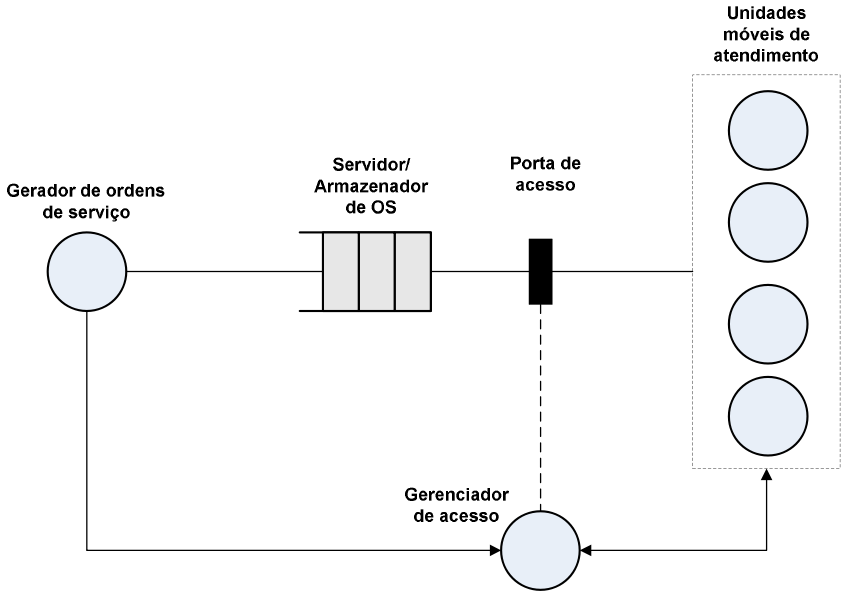
\includegraphics[width=10cm]{imagem/q2.png}
\end{figure}

  \begin{itemize}
   \item Projete um aplicativo que simule o funcionamento do sistema de gerenciamento de ordens de serviço considerando que exista um gerador de OS, 
	um gerenciador de acesso, um armazenador de OS e quatro unidades móveis de atendimento.
  \end{itemize}

\newpage

  \item A equipe de engenharia deseja desenvolver um frequencimetro, isto é, um instrumento de medição capaz de obter a freqüência de qualquer sinal 
      periódico adquirido. O instrumento em questão possui uma faixa de operação de 0 a 1KHz,podendo o valor do sinal adquirido estar em qualquer 
      posição da faixa de operação. O frequenciamento a ser projetado possui três canais de aquisição independentes. Neste caso, a equipe da 
      engenharia eletrônica está responsável por projetar o aplicativo que realize a leitura de um sinal periódico e calcule a freqüência do mesmo. 
      A freqüência de cada canal é impressa no display do instrumento a cada 1 segundo. Com base nos conhecimentos adquiridos e nas informações 
      fornecidas:
      \begin{itemize}
       \item Projete a solução em software que implemente as funcionalidades disponibilizadas pelo frequencímetro. A aquisição dos sinais deve ser 
	    realizada a partir de um arquivo de dados fornecido pelo professor. A informação mostrada no display do instrumento deve ter o seguinte 
	    formato:\\
	    CH01: XXX, CH02: XXX, CH03: XXX,\\
	    Em que:\\
	    XXX = Freqüência do sinal amostrado.
      \end{itemize}
  
\newpage

  \item O sistema ABS (Anti-lock Breaking System) é utilizado para evitar o travamento das rodas do veículo e, por conseguinte a distancia de 
      frenagem. Basicamente, o sistema ABS é composto por quatro sensores de velocidade posicionados em cada roda do veículo, uma ECU (Unidade 
      de Controle Eletrônico) e um modulador de pressão controlado pela ECU. Quando o motorista pressiona o pedal do freio, uma pressão é aplicada 
      sobre o sistema de frenagem do veículo para que a velocidade do mesmo possa ser reduzida. Por outro lado, quando ocorre o travamento da roda 
      (isto é o deslizamento sobre a superfície de contato) a velocidade da roda travada cai abruptamente em relação as demais o que leva ao aumento 
      da distância de frenagem e, em alguns casos, a perda de controle sobre o veículo. O sistema ABS trabalha verificando constantemente a condição 
      de travamento para cada roda. Quando esta condição é verificada, a pressão de frenagem sobre a roda em particular é aliviada momentaneamente 
      para que a roda volte a adquirir velocidade e evite o travamento. Uma vez que a roda volta a adquirir velocidade, a pressão de frenagem sobre 
      a roda é re-estabelecida. A figura abaixo ilustra o diagrama esquemático do sistema ABS.

\begin{figure}[ht]
 \center
 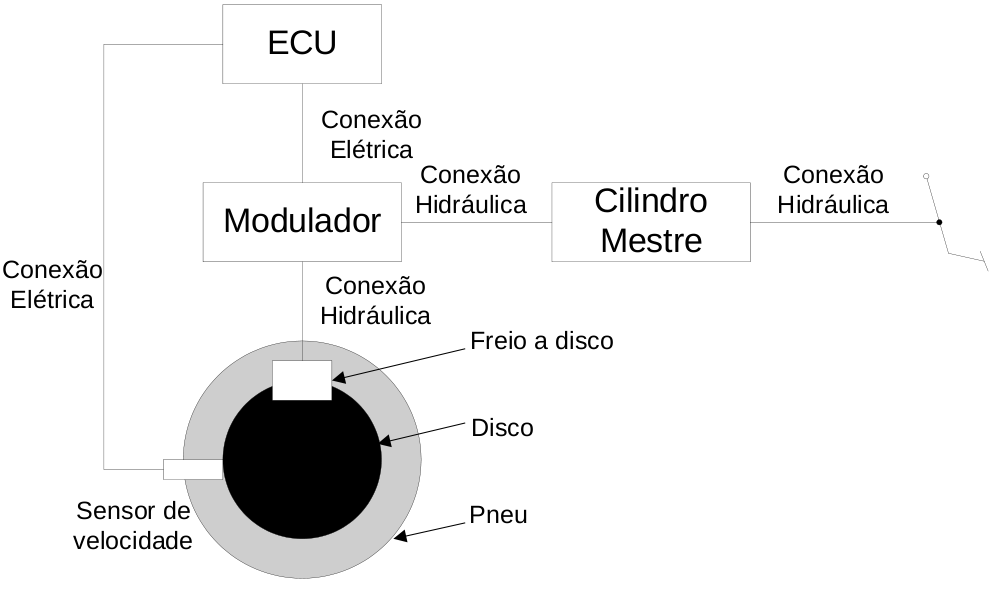
\includegraphics[width=10cm]{imagem/abs.png}
\end{figure}

  Com base nas informações fornecidas:\\
  \begin{itemize}
   \item Projete o controlador lógico do sistema ABS com base nas informações fornecidas. Um arquivo de dados será fornecido pelo professor para 
	indicar a velocidade instantânea de cada roda do veículo. A aquisição do sinal de velocidade deve ser periódica de período (100ms). Imprima 
	no terminal e em um arquivo de dados (controle.txt) a velocidade instantânea de cada roda e as ações do sistema ABS no seguinte formato:\\
	FL:XXX, FR:XXX, RL: XXX, RR: XXX| K: FL, K: FR, K: RL, K: RR\\
	Em que:\\
	FL (Front Left) = Roda dianteira esquerda;\\
	XXX = Velocidade instantânea da roda;\\
	FR (Front Right) = Roda dianteira direita;\\
	RL (Rear Left) = Roda traseira esquerda;\\
	RR (Rear Right) = Roda traseira direita;\\
	K (Ação de controle) = F (Roda livre) ou B(Roda em frenagem);\\
	Obs.: Um arquivo de dados será fornecido pelo professor para indicar a velocidade instantânea de cada roda do veiculo.\\

  \end{itemize}


\end{enumerate}

\end{document}
